% Options for packages loaded elsewhere
\PassOptionsToPackage{unicode}{hyperref}
\PassOptionsToPackage{hyphens}{url}
%
\documentclass[
]{article}
\title{Data Visualisation plots}
\author{}
\date{\vspace{-2.5em}}

\usepackage{amsmath,amssymb}
\usepackage{lmodern}
\usepackage{iftex}
\ifPDFTeX
  \usepackage[T1]{fontenc}
  \usepackage[utf8]{inputenc}
  \usepackage{textcomp} % provide euro and other symbols
\else % if luatex or xetex
  \usepackage{unicode-math}
  \defaultfontfeatures{Scale=MatchLowercase}
  \defaultfontfeatures[\rmfamily]{Ligatures=TeX,Scale=1}
\fi
% Use upquote if available, for straight quotes in verbatim environments
\IfFileExists{upquote.sty}{\usepackage{upquote}}{}
\IfFileExists{microtype.sty}{% use microtype if available
  \usepackage[]{microtype}
  \UseMicrotypeSet[protrusion]{basicmath} % disable protrusion for tt fonts
}{}
\makeatletter
\@ifundefined{KOMAClassName}{% if non-KOMA class
  \IfFileExists{parskip.sty}{%
    \usepackage{parskip}
  }{% else
    \setlength{\parindent}{0pt}
    \setlength{\parskip}{6pt plus 2pt minus 1pt}}
}{% if KOMA class
  \KOMAoptions{parskip=half}}
\makeatother
\usepackage{xcolor}
\IfFileExists{xurl.sty}{\usepackage{xurl}}{} % add URL line breaks if available
\IfFileExists{bookmark.sty}{\usepackage{bookmark}}{\usepackage{hyperref}}
\hypersetup{
  pdftitle={Data Visualisation plots},
  hidelinks,
  pdfcreator={LaTeX via pandoc}}
\urlstyle{same} % disable monospaced font for URLs
\usepackage[margin=1in]{geometry}
\usepackage{graphicx}
\makeatletter
\def\maxwidth{\ifdim\Gin@nat@width>\linewidth\linewidth\else\Gin@nat@width\fi}
\def\maxheight{\ifdim\Gin@nat@height>\textheight\textheight\else\Gin@nat@height\fi}
\makeatother
% Scale images if necessary, so that they will not overflow the page
% margins by default, and it is still possible to overwrite the defaults
% using explicit options in \includegraphics[width, height, ...]{}
\setkeys{Gin}{width=\maxwidth,height=\maxheight,keepaspectratio}
% Set default figure placement to htbp
\makeatletter
\def\fps@figure{htbp}
\makeatother
\setlength{\emergencystretch}{3em} % prevent overfull lines
\providecommand{\tightlist}{%
  \setlength{\itemsep}{0pt}\setlength{\parskip}{0pt}}
\setcounter{secnumdepth}{-\maxdimen} % remove section numbering
\usepackage{booktabs}
\usepackage{longtable}
\usepackage{array}
\usepackage{multirow}
\usepackage{wrapfig}
\usepackage{float}
\usepackage{colortbl}
\usepackage{pdflscape}
\usepackage{tabu}
\usepackage{threeparttable}
\usepackage{threeparttablex}
\usepackage[normalem]{ulem}
\usepackage{makecell}
\usepackage{xcolor}
\ifLuaTeX
  \usepackage{selnolig}  % disable illegal ligatures
\fi

\begin{document}
\maketitle

\hypertarget{experiment-1}{%
\subsection{Experiment 1}\label{experiment-1}}

\hypertarget{egg-counting}{%
\subsubsection{Egg counting}\label{egg-counting}}

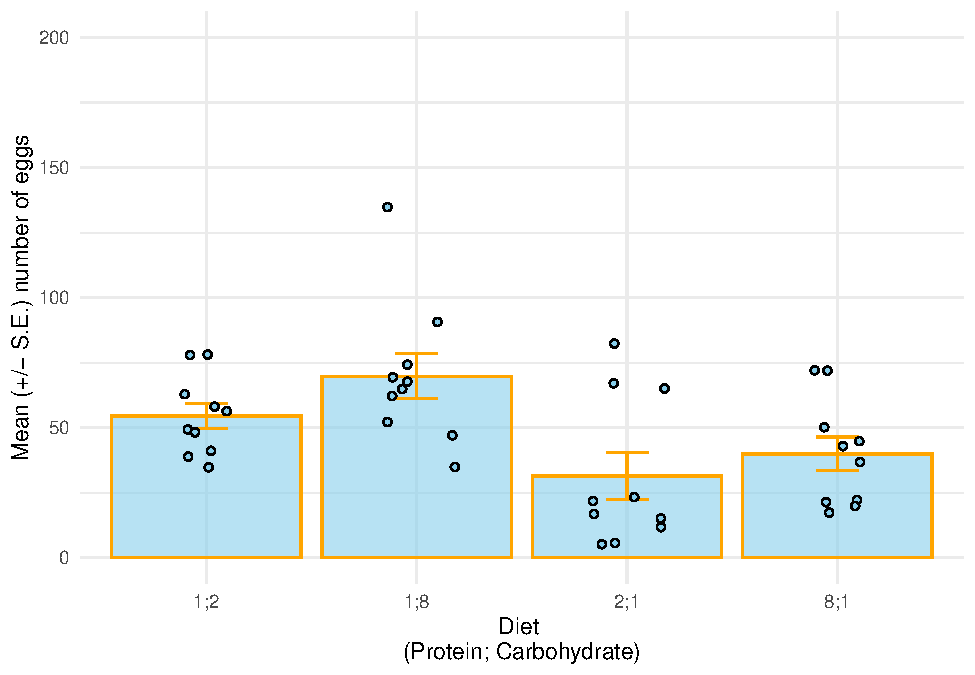
\includegraphics{Drosophila-project_files/figure-latex/unnamed-chunk-2-1.pdf}

\hypertarget{the-number-of-eggs-laid-by-female-flies-across-4-diets}{%
\paragraph{The number of eggs laid by female flies across 4
diets}\label{the-number-of-eggs-laid-by-female-flies-across-4-diets}}

\hypertarget{feeding-behaviour}{%
\subsubsection{Feeding behaviour}\label{feeding-behaviour}}

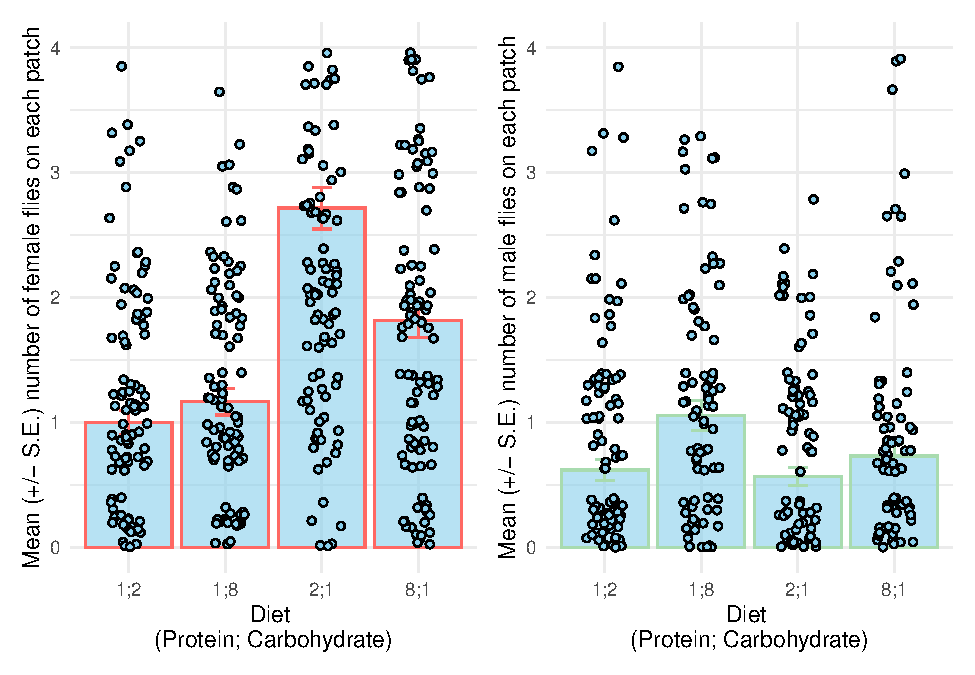
\includegraphics{Drosophila-project_files/figure-latex/unnamed-chunk-3-1.pdf}

\hypertarget{the-mean-average-number-of-flies-feeding-on-diets-across-2-days-females-shown-in-red-and-males-shown-in-blue}{%
\paragraph{The mean average number of flies feeding on diets across 2
days, females (shown in red) and males (shown in
blue)}\label{the-mean-average-number-of-flies-feeding-on-diets-across-2-days-females-shown-in-red-and-males-shown-in-blue}}

\hypertarget{not-feeding}{%
\subsubsection{Not feeding}\label{not-feeding}}

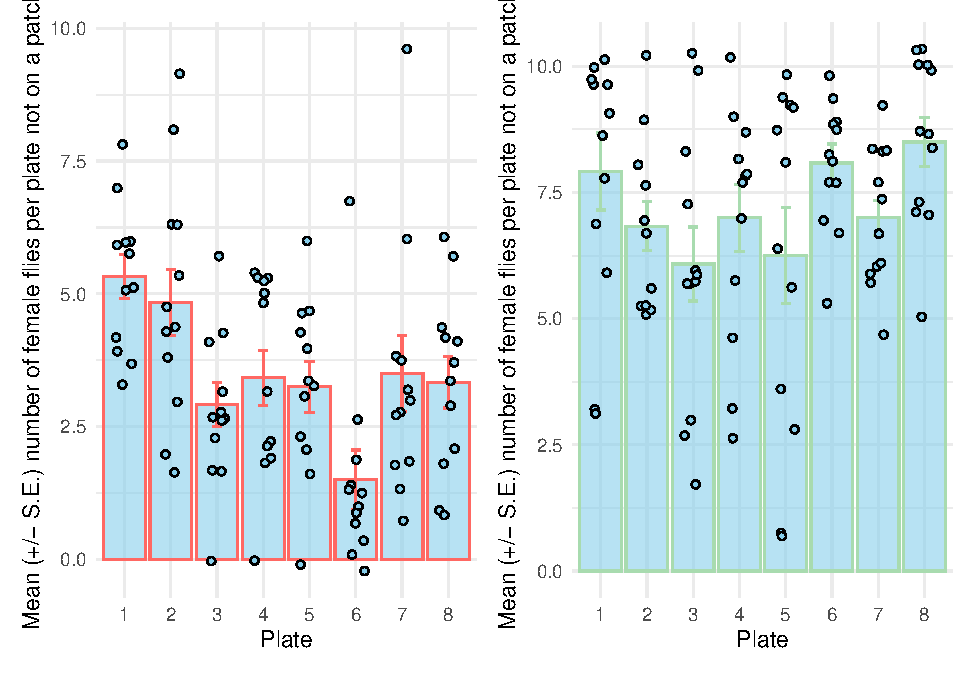
\includegraphics{Drosophila-project_files/figure-latex/unnamed-chunk-4-1.pdf}

\hypertarget{the-mean-average-number-of-flies-not-feeding-on-diets-across-2-days-females-shown-in-red-and-males-shown-in-blue}{%
\paragraph{The mean average number of flies NOT feeding on diets across
2 days, females (shown in red) and males (shown in
blue)}\label{the-mean-average-number-of-flies-not-feeding-on-diets-across-2-days-females-shown-in-red-and-males-shown-in-blue}}

\hypertarget{experiment-2a}{%
\subsection{Experiment 2a}\label{experiment-2a}}

\hypertarget{egg-counting-1}{%
\subsubsection{Egg counting}\label{egg-counting-1}}

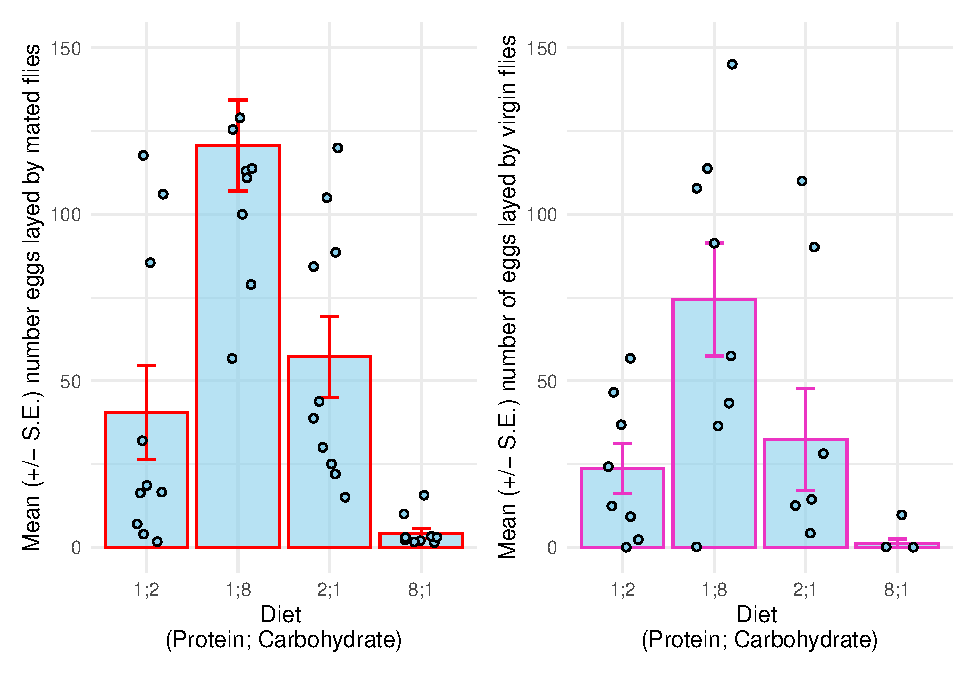
\includegraphics{Drosophila-project_files/figure-latex/unnamed-chunk-5-1.pdf}

\hypertarget{the-mean-average-of-eggs-across-four-diet-ratios-with-mated-females-shown-in-red-and-virgin-females-shown-in-purple}{%
\paragraph{The mean average of eggs across four diet ratios with mated
females (shown in red) and virgin females (shown in
purple)}\label{the-mean-average-of-eggs-across-four-diet-ratios-with-mated-females-shown-in-red-and-virgin-females-shown-in-purple}}

\hypertarget{feeding-behaviour-1}{%
\subsubsection{Feeding behaviour}\label{feeding-behaviour-1}}

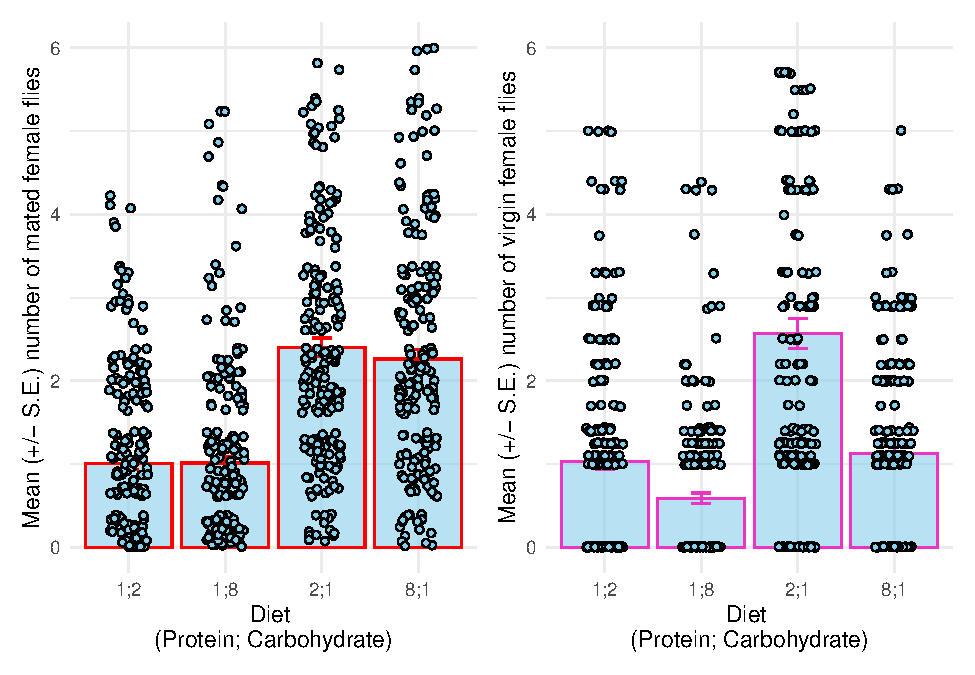
\includegraphics{Drosophila-project_files/figure-latex/unnamed-chunk-6-1.pdf}

\hypertarget{the-mean-average-number-of-flies-feeding-on-diets-across-3-days-mated-females-shown-in-red-and-virgin-females-shown-in-pink}{%
\paragraph{The mean average number of flies feeding on diets across 3
days, mated females (shown in red) and virgin females (shown in
pink)}\label{the-mean-average-number-of-flies-feeding-on-diets-across-3-days-mated-females-shown-in-red-and-virgin-females-shown-in-pink}}

\hypertarget{experiment-2b}{%
\subsection{Experiment 2b}\label{experiment-2b}}

\hypertarget{feeding-behaviour-2}{%
\subsubsection{Feeding behaviour}\label{feeding-behaviour-2}}

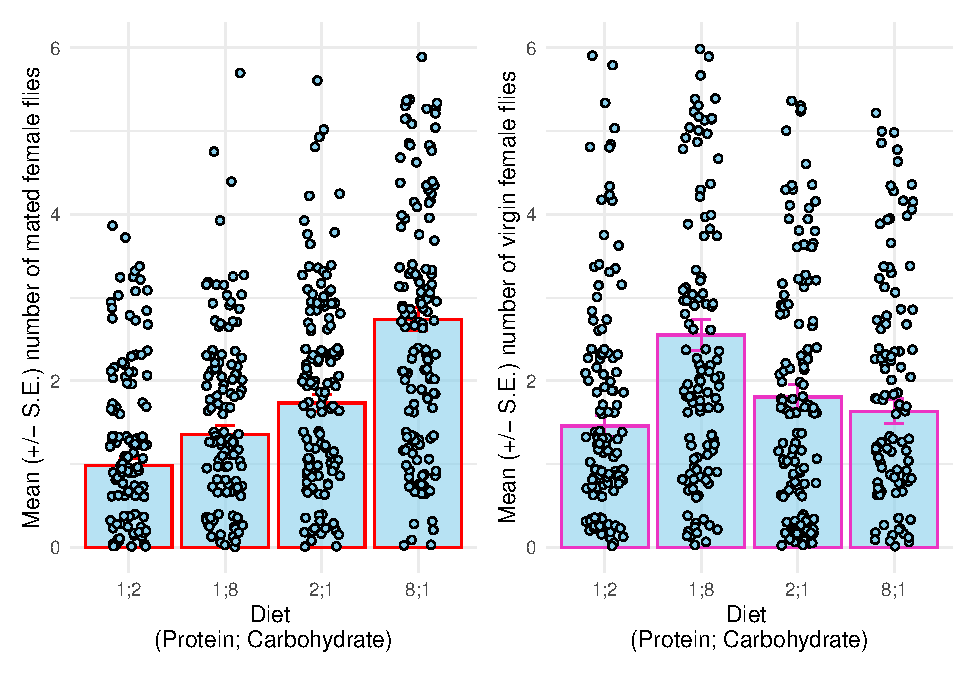
\includegraphics{Drosophila-project_files/figure-latex/unnamed-chunk-7-1.pdf}

\hypertarget{the-mean-average-number-of-flies-feeding-on-diets-across-2-days-mated-females-shown-in-red-and-virgin-females-shown-in-pink}{%
\paragraph{The mean average number of flies feeding on diets across 2
days, mated females (shown in red) and virgin females (shown in
pink)}\label{the-mean-average-number-of-flies-feeding-on-diets-across-2-days-mated-females-shown-in-red-and-virgin-females-shown-in-pink}}

\hypertarget{experiment-3}{%
\subsection{Experiment 3}\label{experiment-3}}

\hypertarget{feeding-behaviour-3}{%
\subsubsection{Feeding behaviour}\label{feeding-behaviour-3}}

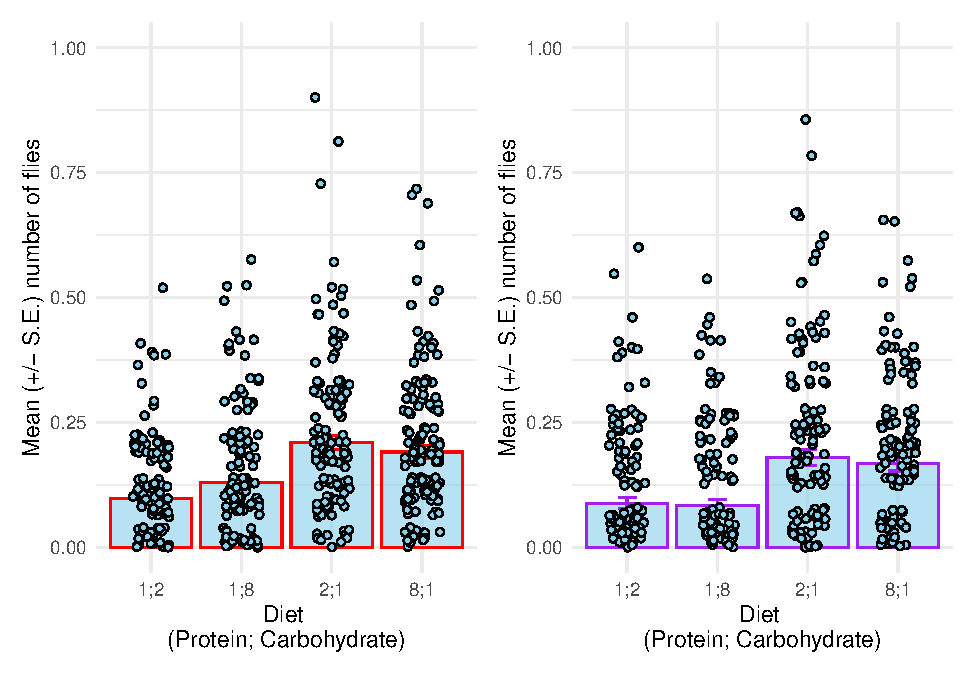
\includegraphics{Drosophila-project_files/figure-latex/unnamed-chunk-8-1.pdf}

\hypertarget{the-calculated-proportional-value-of-the-mean-average-number-of-flies-feeding-on-diets-across-2-days-just-mated-females-alone-on-a-plate-shown-in-red-and-mated-females-along-with-males-on-a-plate-shown-in-purple}{%
\paragraph{The calculated proportional value of the mean average number
of flies feeding on diets across 2 days, just mated females alone on a
plate (shown in red) and mated females along with males on a plate
(shown in
purple)}\label{the-calculated-proportional-value-of-the-mean-average-number-of-flies-feeding-on-diets-across-2-days-just-mated-females-alone-on-a-plate-shown-in-red-and-mated-females-along-with-males-on-a-plate-shown-in-purple}}

There was a strong significant difference when looking at the
interaction effect between diet choice and male and female sex (F =
30.5, P = \textless0.001 ), so this was kept in the model.

There was a significant difference (P = 0.02) found between the diets
that females chose to feed on and the diets that males chose to feed on.
With the 2:1 diet being the most popular diets for females to feed on
with having a mean average of 2.72 flies on a feeding patch at one
observation taken over 2 days of observations. While the most popular
feeding diet for males was 1:8 with there being a mean average of 1.06
flies on a patch at an observation.

There was a large significant difference (P=\textless0.001) found
between females choosing a 1:2 diet (a diet higher in carbohydrate),
than males choosing a 2:1 diet (a diet high in protein).

\end{document}
